\documentclass[aspectratio=169]{beamer}
\usetheme{AnnArbor} %{Madrid} %tema do slide. Tem muitos temas existentes... Gosto desse! Se vcs quiserem mais temas, visitem: http://deic.uab.es/~iblanes/beamer_gallery/index_by_theme.html
\usecolortheme{beaver}
\usepackage[brazil]{babel} %texto
\usepackage[utf8]{inputenc} %texto
\usepackage{graphicx} %imagem	
\usepackage{caption} %imagem
\usepackage{subcaption} %imagem
\usepackage{float} %imagem e tabelas
\usepackage{booktabs} %tabelas	
\usepackage[abnt-emphasize=bf,alf]{abntex2cite} %citacoes ABNT
\usepackage{verbatim}
\graphicspath{{./Figuras/}} %Colarimages na pasta "Figuras". Gosto de fazer isso para organizar os arquivos.    		

%---------------------------------------------------------------------------
	% PRIMEIRA SECAO
	\section{Centro Federal de Educação Tecnológica de Minas Gerais}
	\subsection{Curso Técnico em Mecatrônica}
%---------------------------------------------------------------------------

\begin{document}
	% EDITAR ESSAS INFORMACOES (INICIO)
	\title[3º Relatório de Acompanhamento do Estagiário]{QUALIDADE E REPARO EM PROCESSOS INDUSTRIAIS DE GRANDE ESCALA}
	\subtitle{Aplicado a SmartPhones}
	\author[antonioaads@gmail.com]{Antônio Augusto Diniz Sousa}
	\institute[]{CEFET-MG}
	\date[2017]{\today}
	% EDITAR ESSAS INFORMACOES (FIM)
	
	\begin{frame}
		\titlepage
	\end{frame}
	\begin{frame}
		\frametitle{Sum\'{a}rio}
		\tableofcontents%[pausesections]
	\end{frame}
	
%---------------------------------------------------------------------------
	% PRIMEIRA SECAO
	\section{Global Express}
	\subsection{A empresa}
%---------------------------------------------------------------------------
	
	% SLIDE 1 - Introdução	
	\begin{frame}
		\frametitle{Global Express}
		\framesubtitle{Serviços}
		
		\begin{minipage}[!h]{.4\textwidth}
			\begin{itemize}
				\item \textit{Assistência Técnica Especializada};
				\begin{itemize}
					\item \textit{\textbf{SmartPhones}}
					\item \textit{SmartWatch}
					\item \textit{Óculos de realidade virtual}
					\item \textit{Câmeras (360)}
				\end{itemize}
			\end{itemize}
		\end{minipage}
		\hfill
		\begin{minipage}[!h]{.5\textwidth}
			\begin{figure}
				\centering
				\caption{Logo da Global Express}
				
				
\includegraphics[width=.70\linewidth]{logo_global.png}
				
				\footnotesize{Fonte: \citeonline{global}}
				\label{logglob}
			\end{figure} 	 
		\end{minipage}
	\end{frame}
	
	% SLIDE 2 - EMPRESAS	
	\begin{frame}
		\frametitle{Terceirização de Serviço}
		\framesubtitle{Samsung, Sony e Microsoft}
		
		\begin{minipage}[!h]{.3\textwidth}
			\begin{itemize}
				\item \textit{Empresas};
				\begin{itemize}
					\item \textit{Microsoft}
					\item \textit{Sony}
					\item \textit{\textbf{Samsung}}
				\end{itemize}
			\end{itemize}
		\end{minipage}
		\hfill
		\begin{minipage}[!h]{.3\textwidth}
			\begin{figure}
				\centering
				\caption{Logo da Samsung}
				
				
\includegraphics[width=.90\linewidth]{logo_samsung.png}
				
				\footnotesize{Fonte: \citeonline{samsung}}
				\label{logsam}
			\end{figure} 	 
		\end{minipage}
		\hfill	
		\begin{minipage}[!h]{.3\textwidth}
			\begin{figure}
				\centering
				\caption{Logo da Sony}
				
				
\includegraphics[width=.65\linewidth]{logo_sony.png}
				
				\footnotesize{Fonte: \citeonline{sony}}
				\label{logsony}
				
				\centering
				\caption{Logo da Microsoft}
				
				
\includegraphics[width=.65\linewidth]{logo_microsoft.png}
				
				\footnotesize{Fonte: \citeonline{microsoft}}
				\label{logmicro}
			\end{figure} 	
		\end{minipage}
	\end{frame}
	
	% SLIDE 3 - DEPARTAMENTOS
	\begin{frame}
		\frametitle{Departamentos}
		\framesubtitle{Organograma}
		
		\begin{figure}
			\centering
			\caption{Organograma Global Express}
			
			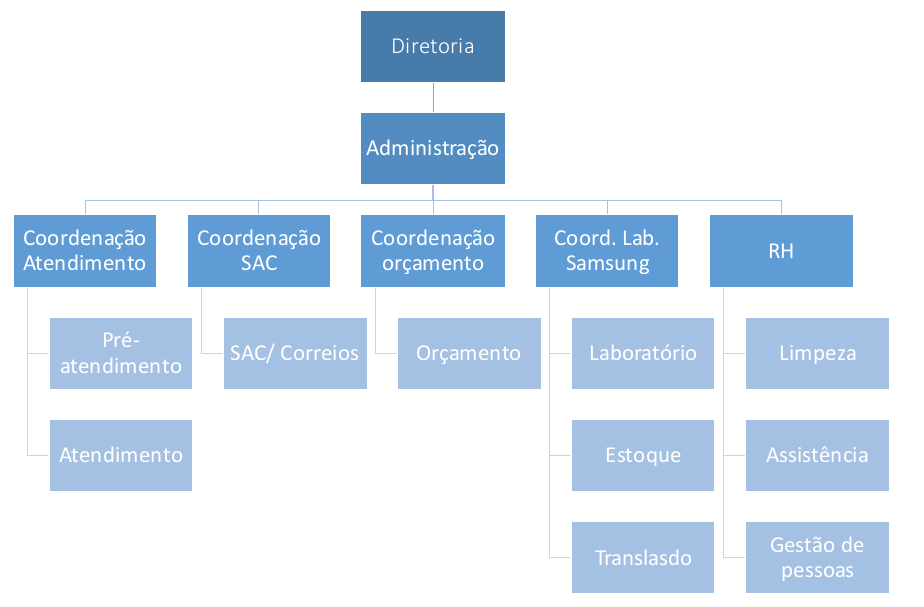
\includegraphics[width=0.5	\linewidth]{organograma_global.png} 
			
			\footnotesize{Fonte: Autor}
			\label{im1}
		\end{figure}	
	\end{frame}
	
	% SLIDE 4 - Fluxograma	
	\begin{frame}
		\frametitle{Fluxograma}
		\framesubtitle{Processos entre envio e recebimento do produto}
		
		\begin{minipage}[H]{.3\textwidth}
			\begin{itemize}
				\item \textit{Cliente};
				\item \textit{Atendimento/SAC};
				\item \textit{Translado};
				\item \textit{\textbf{Laboratório}};
				\item \textit{Estoque};
				\item \textit{\textbf{Laboratório}};
				\item \textit{\textbf{OQC}};
				\item \textit{SAC};
				\item \textit{Cliente};
			\end{itemize}
		\end{minipage}
		\hfill
		\begin{minipage}[H]{.65\textwidth}
			\begin{figure}
				\centering
				\caption{Fluxograma Global Express}
			
				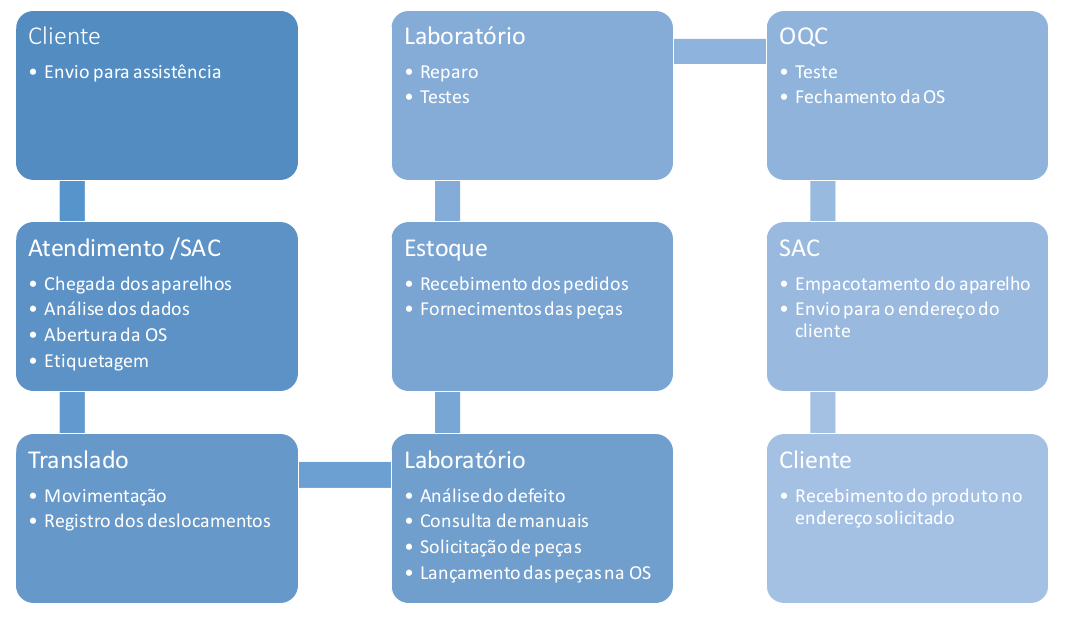
\includegraphics[width=0.8	\linewidth]{fluxograma_global.png} 
			
				\footnotesize{Fonte: Autor}
				\label{im1}
			\end{figure}
		\end{minipage}
	\end{frame}

%---------------------------------------------------------------------------
	% SEGUNDA SECAO
	\subsection{O estagiário}
%---------------------------------------------------------------------------
	% SLIDE 5 - Intodução Estagiário	
	\begin{frame}
		\frametitle{O estagiário}
		\framesubtitle{Como foi o estágio...}
		
		\begin{minipage}[H]{.3\textwidth}
			\begin{itemize}
				\item \textit{Apresentação da empresa};
				\begin{itemize}
					\item \textit{Espaços da empresa}
					\item \textit{Normas e regras}
					\item \textit{Segurança}
					\item \textit{Organização}
					\item \textit{Processo}
					\item \textit{Observação (1 mês)}
				\end{itemize}
			\end{itemize}
		\end{minipage}
		\hfill
		\begin{minipage}[H]{.3\textwidth}
			\begin{itemize}
				\item \textit{OQC};
				\begin{itemize}
					\item \textit{Auxílio}
					\item \textit{Meta}
					\item \textit{Produção}
					\item \textit{Trabalho Individual}
					\item \textit{Cobrança}
				\end{itemize}
			\end{itemize}
		\end{minipage}
		\hfill
		\begin{minipage}[H]{.3\textwidth}
			\begin{itemize}
				\item \textit{Laboratório};
				\begin{itemize}
					\item \textit{Auxílio}
					\item \textit{Segurança - ESD}
					\item \textit{Manutenção}
					\item \textit{Responsabilidade}
					\item \textit{Trabalho Individual}
					\item \textit{Cobrança*}
				\end{itemize}
			\end{itemize}
		\end{minipage}
	\end{frame}
	
	%---------------------------------------------------------------------------
	% SEGUNDA SECAO
	\section{SAMSUNG}
	\subsection{Monitoria}
%---------------------------------------------------------------------------
	% SLIDE 5 - Intodução Estagiário	
	\begin{frame}
		\frametitle{SAMSUNG}
		\framesubtitle{Análise, Inspeção e Controle}
		
		\begin{minipage}[H]{.4\textwidth}
			\begin{itemize}
				\item \textit{GSPN};
				\begin{itemize}
					\item \textit{Controle}
					\item \textit{Qualidade}
					\item \textit{Serviços}
					\item \textit{Treinamentos}
				\end{itemize}
			\end{itemize}
		\end{minipage}
		\hfill
		\begin{minipage}[H]{.4\textwidth}
			\begin{itemize}
				\item \textit{Visitas Técnicas};
				\begin{itemize}
					\item \textit{Monitoramento}
					\item \textit{Pesquisa (motivos)}
					\item \textit{Inspeção}
					\item \textit{Análise de processo}
					\item \textit{Acompanhamento}
				\end{itemize}
			\end{itemize}
		\end{minipage}
		\hfill
		\begin{minipage}[H]{.4\textwidth}
			\begin{itemize}
				\item \textit{Fábrica};
				\begin{itemize}
					\item \textit{Recolhimento}
					\item \textit{Documentação}
					\item \textit{Dicas de Reparo}
					\item \textit{Defeitos de fabricação}
				\end{itemize}
			\end{itemize}
		\end{minipage}
	\end{frame}
	
	\begin{comment}
	% SLIDE 1 - UMA TABELA	
	\begin{frame}
		\frametitle{Tabelas}
				
		\begin{table}[H]
			\centering
			\caption{Atributos dos arquivos}
			\begin{tabular}{c|c}
				\toprule
				\textbf{Atributo} & \textbf{Significado} \\
				\midrule
				Prote\c{c}\~{a}o&Quem tem acesso ao arquivo e de que modo\\
				\midrule
				Senha&Necessidade de senha para acesso ao arquivo\\
				\midrule
				Criador&ID do criador do arquivo\\
				\midrule
				Propriet\'{a}rio&Propriet\'{a}rio atual\\
				\bottomrule
			\end{tabular}
			
			\label{tab:attI}
			\footnotesize{Fonte: \citeonline{tanebaun2010}}				
		\end{table}
	\end{frame}
%---------------------------------------------------------------------------

	% SLIDE 1 - APENAS UMA IMAGEM	
	\begin{frame}
		\frametitle{Global Express}
		\framesubtitle{A empresa}
		Imagine a Figura:
		
		\begin{figure}
			\centering
			\caption{Legenda da figura}
			
			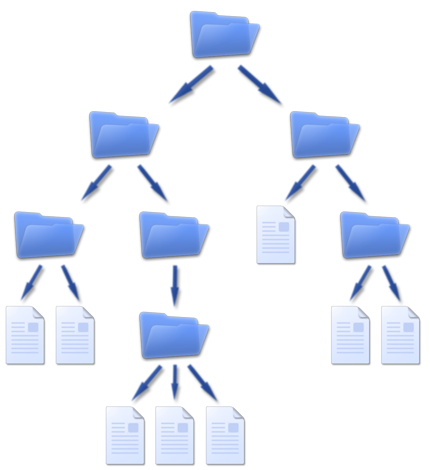
\includegraphics[width=.25\linewidth]{sa.png} 
			
			\footnotesize{Fonte: ...	
				\par Visitado em \today.}
			\label{im1}
		\end{figure}	
	\end{frame}
	
	% SLIDE 2 - APENAS UMA IMAGEM	
	\begin{frame}
		\frametitle{Imagem}
		\framesubtitle{Imagens simples sem legenda}
			Imagine a Figura:
		
			\center
			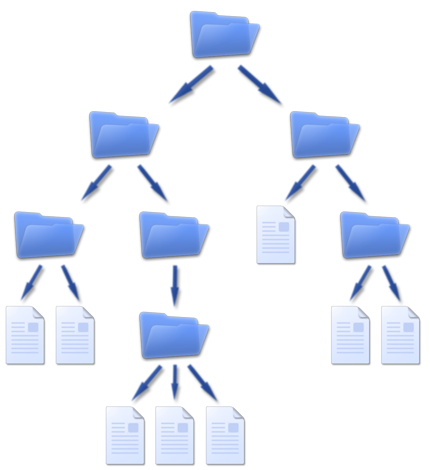
\includegraphics[width=.25\linewidth]{sa.png} 	
	\end{frame}
	
	% SLIDE 3 - TEXTO SEGUIDO DE UMA IMAGEM	
	\begin{frame}
		\frametitle{Imagem}
		\framesubtitle{Imagens agrupadas}
		Imagine a Figura:
		
		\begin{figure}[H]
			\centering
			\caption{Legenda da figura}
			\begin{subfigure}{0.45\textwidth}
				\centering
				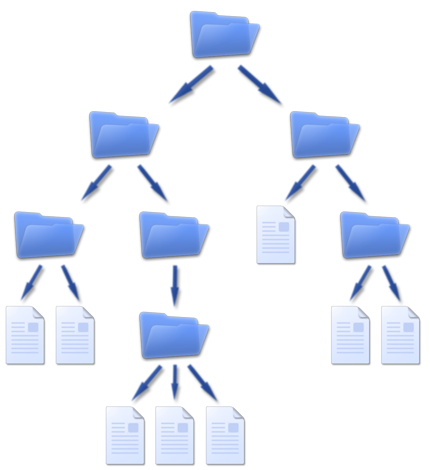
\includegraphics[width=.25\linewidth]{sa.png}
				\caption{Legenda da parte 1}
				\label{figPt1}
			\end{subfigure}
			\hfill
			\begin{subfigure}{0.45\textwidth}
				\centering
				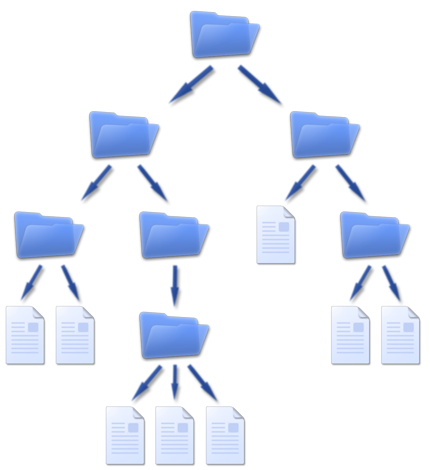
\includegraphics[width=.25\linewidth]{sa.png}
				\caption{Legenda da parte 2}
				\label{figPt2}
			\end{subfigure}                                                   
			
			\footnotesize{Fonte: \citeonline{tanebaun2010}}
			\label{figPt1e2}
		\end{figure}	
	\end{frame}
	
	% SLIDE 4 - TEXTO EM UMA COLUNA, IMAGEM EM OUTRA COLUNA	
	\begin{frame}
		\frametitle{Imagem}
		\framesubtitle{Imagem e texto}
		
		\begin{minipage}[H]{.5\textwidth}
			Texto texto texto texto texto texto texto texto texto texto texto texto texto texto texto texto texto texto texto texto texto texto texto texto texto texto texto texto texto texto texto texto texto texto texto texto texto texto texto texto texto texto texto texto texto texto texto texto texto texto texto texto texto texto texto texto texto texto texto texto texto texto texto texto texto texto texto texto texto texto texto texto texto texto texto texto texto texto texto texto texto texto texto texto texto texto texto.	
		\end{minipage}
		\hfill
		\begin{minipage}[H]{.45\textwidth}
			\begin{figure}
				\centering
				\caption{Legenda da imagem}
				
				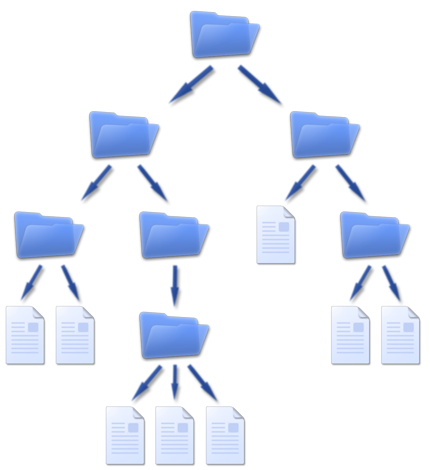
\includegraphics[width=.25\linewidth]{sa.png}
				
				\footnotesize{Fonte: \citeonline{tanebaun2010}}
				\label{figtextimg}
			\end{figure}  
		\end{minipage}
	\end{frame}
	
%---------------------------------------------------------------------------
	% SEGUNDA SECAO
	\section{Tabelas}	
%---------------------------------------------------------------------------
	% SLIDE 5 - UMA TABELA	
	\begin{frame}
		\frametitle{Tabelas}
				
		\begin{table}[H]
			\centering
			\caption{Atributos dos arquivos}
			\begin{tabular}{c|c}
				\toprule
				\textbf{Atributo} & \textbf{Significado} \\
				\midrule
				Prote\c{c}\~{a}o&Quem tem acesso ao arquivo e de que modo\\
				\midrule
				Senha&Necessidade de senha para acesso ao arquivo\\
				\midrule
				Criador&ID do criador do arquivo\\
				\midrule
				Propriet\'{a}rio&Propriet\'{a}rio atual\\
				\bottomrule
			\end{tabular}
			
			\label{tab:attI}
			\footnotesize{Fonte: \citeonline{tanebaun2010}}				
		\end{table}
	\end{frame}
	
%---------------------------------------------------------------------------
	% TERCEIRA SECAO
	\section{Listas}
%---------------------------------------------------------------------------
	% SLIDE 6 - LISTAGEM SIMPLES
	\begin{frame}
		\frametitle{Listas}
		\framesubtitle{Listas Simples}
		\begin{itemize}
			\item \textit{Create};
			\item \textit{Delete};
			\item \textit{Open};
			\item \textit{Close};
			\item \textit{Read};
		\end{itemize}
	\end{frame}
	
	% SLIDE 7 - LISTAS E SUBLISTAS
	\begin{frame}
		\frametitle{Listas}
		\framesubtitle{Listas e sublistas}
		\begin{itemize}
			\item \textit{Create};
			\begin{itemize}
				\item \textit{Open};
				\item \textit{Close};
				\item \textit{Read};
			\end{itemize}
			\item \textit{Delete};
			
		\end{itemize}
	\end{frame}
	
\end{comment}
	
%---------------------------------------------------------------------------
	%SECAO DE REFERENCIAS
	\section{Refer\^{e}ncias bibliogr\'{a}ficas}
%---------------------------------------------------------------------------
\begin{comment}	
	% SLIDE 8 - REFERENCIAS
	\begin{frame}
		\frametitle{Refer\^{e}ncias bibliogr\'{a}ficas indiretas}
		\textbackslash citeonline\{labelDaReferencia\}\\
		\textbf{Resultado}: De acordo com \citeonline{tanebaun2010}, os computadores...
	\end{frame}
		
	% SLIDE 9 - REFERENCIAS
	\begin{frame}
		\frametitle{Refer\^{e}ncias bibliogr\'{a}ficas diretas}
		\textbackslash cite[p. \~{}45]\{labelDaReferencia\} \\
		\textbf{Resultado}: "os computadores..." \cite[p.~45]{tanebaun2010} 
	\end{frame}	
\end{comment}
	% SLIDE 10 - REFERENCIAS
	\begin{frame}
		%[allowframebreaks]
		\frametitle{Refer\^{e}ncias bibliogr\'{a}ficas}
		\bibliography{Referencias}
	\end{frame}
	%---------------------------------------------------------------------------
\end{document}
